\section{PDDL definition}
\label{sec:pddl}

\subsection{Catching mice}



\begin{multicols}{2}

\begin{figure}[H]
    \centering
    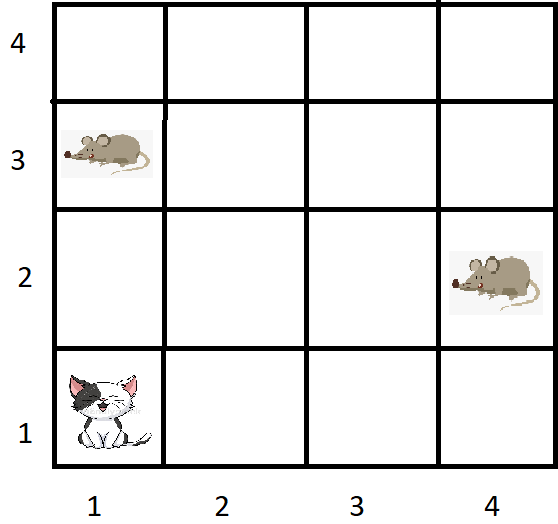
\includegraphics[width=\linewidth]{fig/A3/cat_01.png}
    \caption{\textbf{Problem 1:} Catching two mice}
    \label{fig:cat_01}
\end{figure}

\columnbreak

\begin{figure}[H]
    \centering
    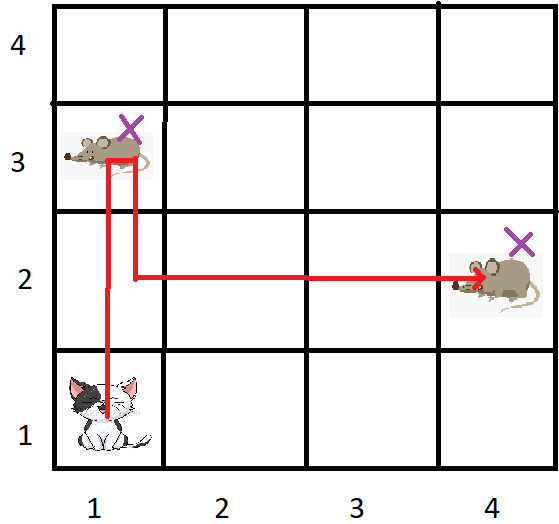
\includegraphics[width=\linewidth]{fig/A3/cat_01_sol.png}
    \caption{\textbf{Plan for problem 1:} The red line shows the trajectory of the cat. The purple 'x' marks that the cat ate the mouse}
    \label{fig:cat_01_sol}
\end{figure}

\end{multicols}

The first step to solve the problem is to define the two fundamental actions the cat can take: moving to neighboring rooms and eating a mouse.


\subsubsection{Domain}

The first types of the domain represent the type of elements that can be inside a room: cat and mouse. The square type represents a room, identified by the row and column indices.

The \verb|at| predicate shows whether an object is inside a given room or not. The \verb|adj| predicate indicates whether two squares are adjacent or not. Finally the \verb|dead| predicate shows whether the given mouse is dead or not.


\lstinputlisting[caption=Domain: types and predicates, linerange=1-8, firstnumber=1]{../planning/cat-eat.pddl}

To move from one square to another, the two squares must be adjacents to each other, and the cat should be inside the first one. Moving means to leave the current square and to enter the next one.

\lstinputlisting[caption=Domain: the move action, linerange=10-20, firstnumber=10]{../planning/cat-eat.pddl}

The cat can eat a mouse when they are both in the same square. Eating a mouse means to remove it from the world and mark it dead.

\lstinputlisting[caption=Domain: the eat action, linerange=22-32, firstnumber=22]{../planning/cat-eat.pddl}


\subsubsection{Problem 1}

The first problem is to catch two mice. There are no constraints besides the rule of moving only to adjacent cells. The initial state can be seen on figure \ref{fig:cat_01}.

The objects that appear in the problem are: a cat, two mice and 16 squares.

\lstinputlisting[caption=Problem 1: objects, linerange=1-11, firstnumber=1]{../planning/cat-p01.pddl}

To describe the initial state, first we must define the adjacency relationship between the squares.

\lstinputlisting[caption=Problem 1: adjacency relationships, linerange=13-38, firstnumber=13]{../planning/cat-p01.pddl}

Then the initial locations of the cat and the mice are specified:

\lstinputlisting[caption=Problem 1: initial locations, linerange=40-45, firstnumber=40]{../planning/cat-p01.pddl}

Finally the goal is defined: to get rid of all the mice.

\lstinputlisting[caption=Problem 1: goal, linerange=48-48, firstnumber=48]{../planning/cat-p01.pddl}


\subsubsection{Result}

One should type the following line to run the example: 

\begin{lstlisting}[numbers=none]
fd cat-eat.pddl cat-p01.pddl --heuristic "h=ff( )" --search "astar(h)"
\end{lstlisting}

The program prints the following solution:

\lstinputlisting[caption=Output plan]{../planning/cat-p01-plan.txt}

Figure \ref{fig:cat_01_sol} visualizes the resulted plan. The cat goes straight to the closest mouse, eats it, than moves on the shortest path to the second one and eats that too.






\subsection{Adding walls}

\begin{figure}[H]
    \centering
    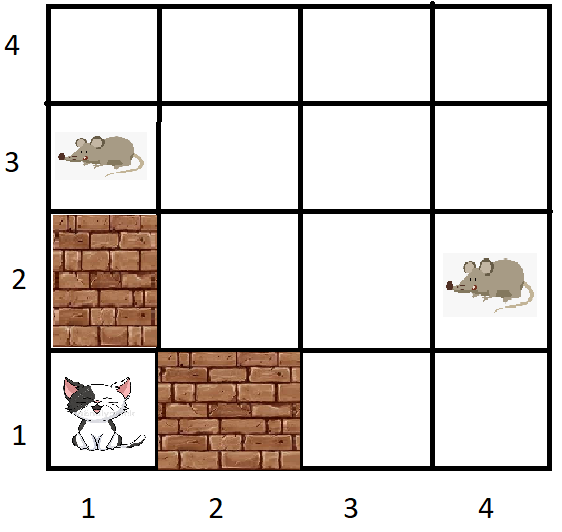
\includegraphics[width=.5\linewidth]{fig/A3/cat_02.png}
    \caption{\textbf{Problem 2:} Two walls completely blocking the cat}
    \label{fig:cat_02}
\end{figure}

The next step of solving the problem is to define walls which block the movement of the cat, forcing it to go around.


\subsubsection{Domain}

A new type must be added for the walls.

\lstinputlisting[caption=Domain: types, linerange=3-3, firstnumber=3]{../planning/cat-wall.pddl}

The precondition of the \verb|move| action must be updated in order to prohibit moving to squares containing walls.

\lstinputlisting[caption=Domain: the move action, linerange=10-21, firstnumber=10]{../planning/cat-wall.pddl}


\subsubsection{Problem 2}

The second problem is to catch two mice while the cat being blocked by two walls. The cat can only move to adjacent cells which don't contain walls. The initial state can be seen on figure \ref{fig:cat_02}.

The objects that appear in the problem are: a cat, two mice, two walls and 16 squares.

\lstinputlisting[caption=Problem 2: objects, linerange=1-12, firstnumber=1]{../planning/cat-p02.pddl}

The initial states of the cat and the mice and the adjacency relationships between the squares are unchanged. The goal is also preserved: to get rid of the two mice. The initial positions of the wall are expressed in the following way:

\lstinputlisting[caption=Problem 2: initial location of the walls, linerange=48-50, firstnumber=48]{../planning/cat-p02.pddl}


\subsubsection{Result}

One should type the following line to run the example: 

\begin{lstlisting}[numbers=none]
fd cat-wall.pddl cat-p02.pddl --heuristic "h=ff( )" --search "astar(h)"
\end{lstlisting}

The program prints the following to the console:

\begin{lstlisting}[numbers=none]
Search stopped without finding a solution.
\end{lstlisting}

One can see on figure \ref{fig:cat_02} that the cat has no possibility to reach the mice, because of being completely blocked by the two walls. The planner program by not providing a solution it verifies that the blocking mechanism is indeed working.


\subsubsection{Problem 3}

\begin{multicols}{2}

\begin{figure}[H]
    \centering
    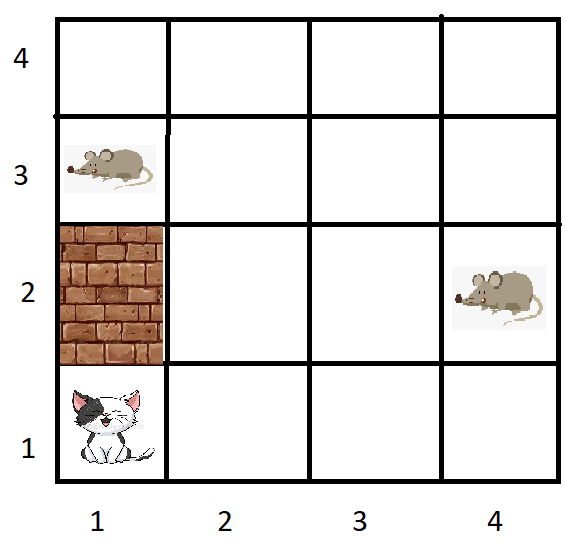
\includegraphics[width=\linewidth]{fig/A3/cat_03.png}
    \caption{\textbf{Problem 3:} Adding walls}
    \label{fig:cat_03}
\end{figure}

\columnbreak

\begin{figure}[H]
    \centering
    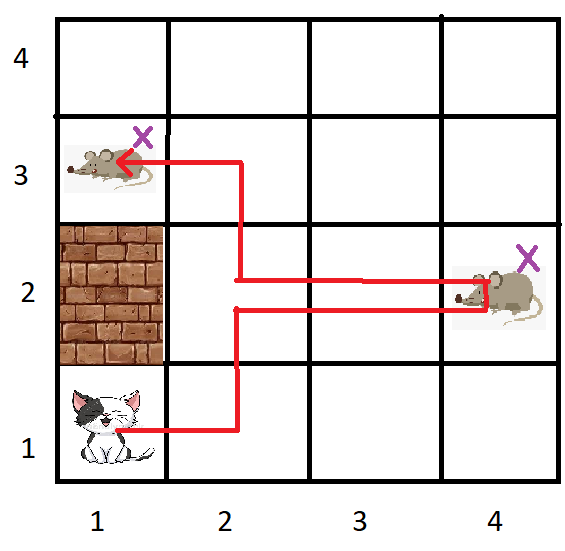
\includegraphics[width=\linewidth]{fig/A3/cat_03_sol.png}
    \caption{\textbf{Plan for problem 3}}
    \label{fig:cat_03_sol}
\end{figure}

\end{multicols}

In this problem we removed the wall from position (1,2) to allow the cat to complete its goal. The problem instance can be seen on figure \ref{fig:cat_03}.

\lstinputlisting[caption=Problem 3: initial location of the wall, linerange=48-50, firstnumber=48]{../planning/cat-p03.pddl}


\subsubsection{Result}

One should type the following line to run the example: 

\begin{lstlisting}[numbers=none]
fd cat-wall.pddl cat-p03.pddl --heuristic "h=ff( )" --search "astar(h)"
\end{lstlisting}

The program prints the following solution:

\lstinputlisting[caption=Output plan]{../planning/cat-p03-plan.txt}

Figure \ref{fig:cat_03_sol} visualizes the resulted plan. The cat goes on the shortest path to position (2,2). At this location it is from the same distance from the two mice. Therefore it can choose both of them as the first victim. The cat chooses the mouse on (2, 4) than goes to (3,1) on the shortest path. 

By comparing the result with the plan at figure \ref{fig:cat_01_sol} one can observe that the shortest path would have been to move straight to the mouse on (3, 1). However now, because of the wall, the cat must go around it. Therefore resulting in a change both in the path and in the plan.









\subsection{Adding traps}

The next step of solving the problem is to define traps which can kill both the cat or the mouse, depending on what lands on them. However these traps are for single use. After a mouse is landed on a trap, the trap becomes disabled and the cat can move freely to that square.


\subsubsection{Domain}

A new type must be added for the traps.

\lstinputlisting[caption=Domain: types, linerange=3-3, firstnumber=3]{../planning/cat-trap.pddl}

The precondition of the \verb|move| action must be updated in order to allow moving only when the cat is alive. Moreover after each move it must be verified if there are any traps on that square or note. If there are no traps, the position of the cat is updated as before. However if the cat lands on a trap, it is removed from the world and marked as dead.

\lstinputlisting[caption=Domain: the move action, linerange=10-23, firstnumber=10]{../planning/cat-trap.pddl}

The precondition of the \verb|eat| action must be updated in order to allow eating only when the cat is alive.

\lstinputlisting[caption=Domain: the eat action, linerange=25-36, firstnumber=25]{../planning/cat-trap.pddl}

Because of inserting in all the preconditions that the cat must not be dead, after the cat dies it can no longer reach the goal, i.e. no more actions can be taken.


\subsubsection{Problem 4}

\begin{multicols}{2}

\begin{figure}[H]
    \centering
    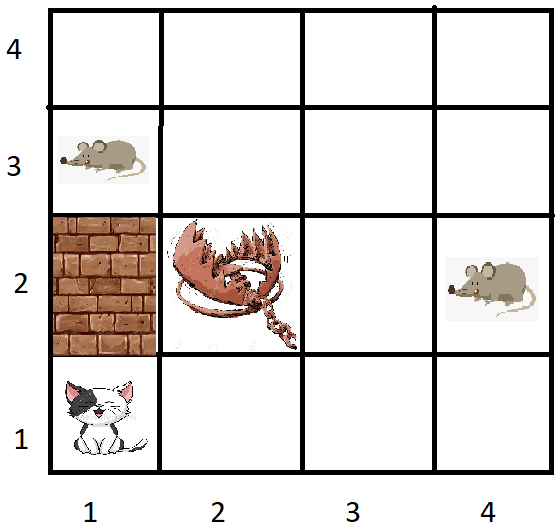
\includegraphics[width=\linewidth]{fig/A3/cat_04.png}
    \caption{\textbf{Problem 4:} Adding traps. The goal of the cat is to die.}
    \label{fig:cat_04}
\end{figure}

\columnbreak

\begin{figure}[H]
    \centering
    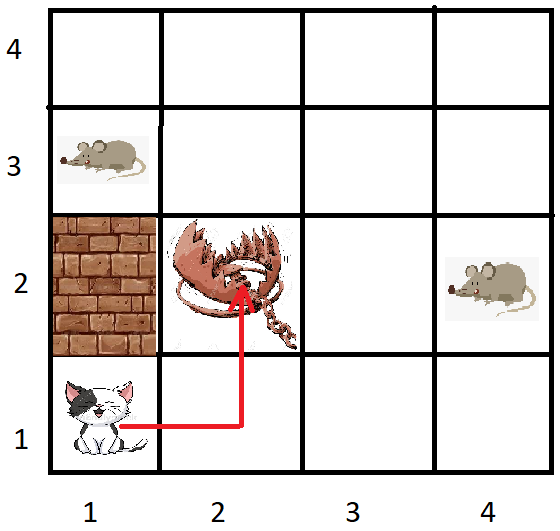
\includegraphics[width=\linewidth]{fig/A3/cat_04_sol.png}
    \caption{\textbf{Plan for problem 4}}
    \label{fig:cat_04_sol}
\end{figure}

\end{multicols}

In this problem a trap was added to position (2,2). The problem instance can be seen on figure \ref{fig:cat_04}. To test the effect of the trap, the goal of this problem is for the cat to die. This can be achieved only by going into the trap.

The objects that appear in the problem are: a cat, two mice, two walls, a trap and 16 squares.

\lstinputlisting[caption=Problem 4: objects, linerange=1-13, firstnumber=1]{../planning/cat-p04.pddl}

The initial states of the cat, the mice and the walls and the adjacency relationships between the squares are unchanged. The initial positions of the wall are expressed in the following way:

\lstinputlisting[caption=Problem 4: initial location of the trap, linerange=52-53, firstnumber=52]{../planning/cat-p04.pddl}


The goal of the problem is for the cat to die:

\lstinputlisting[caption=Problem 4: goal, linerange=56-56, firstnumber=56]{../planning/cat-p04.pddl}


\subsubsection{Result}

One should type the following line to run the example: 

\begin{lstlisting}[numbers=none]
fd cat-trap.pddl cat-p04.pddl --heuristic "h=ff( )" --search "astar(h)"
\end{lstlisting}

The program prints the following solution:

\lstinputlisting[caption=Output plan]{../planning/cat-p04-plan.txt}

Figure \ref{fig:cat_04_sol} visualizes the resulted plan. The cat goes on the shortest path to the trap. Then by dying the goal is reached.



\subsubsection{Problem 5}

\begin{figure}[H]
    \centering
    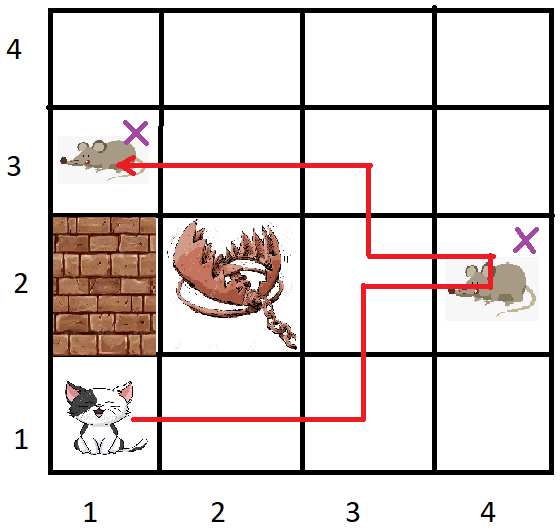
\includegraphics[width=.5\linewidth]{fig/A3/cat_05_sol.png}
    \caption{\textbf{Plan for problem 5:} Eat two mice and be alive}
    \label{fig:cat_05_sol}
\end{figure}

The problem instance is the same as before, can be seen on figure \ref{fig:cat_04}. However the goal is changed back to the previous one: to get rid of all the mice.

\lstinputlisting[caption=Problem 5: goal, linerange=56-56, firstnumber=56]{../planning/cat-p05.pddl}


\subsubsection{Result}

One should type the following line to run the example: 

\begin{lstlisting}[numbers=none]
fd cat-trap.pddl cat-p05.pddl --heuristic "h=ff( )" --search "astar(h)"
\end{lstlisting}

The program prints the following solution:

\lstinputlisting[caption=Output plan]{../planning/cat-p05-plan.txt}

Figure \ref{fig:cat_05_sol} visualizes the resulted plan. The cat must go around the wall and the trap to reach the mouse on (3,1). It goes on a path which reduces the distance toward the two mice. After reaching position (2,3) the cat does a detour to eat the closest mouse. Than it goes on the shortest path to eat the mouse on (3,1).



\subsubsection{Problem 6}

\begin{multicols}{2}

\begin{figure}[H]
    \centering
    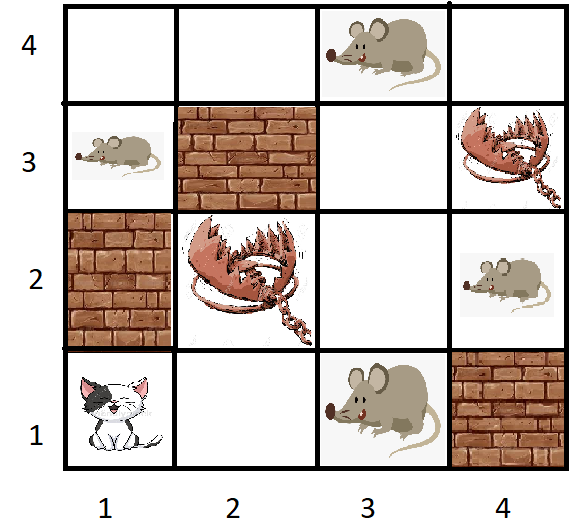
\includegraphics[width=\linewidth]{fig/A3/cat_06.png}
    \caption{\textbf{Problem 6:} Adding more objects to the world}
    \label{fig:cat_06}
\end{figure}

\columnbreak

\begin{figure}[H]
    \centering
    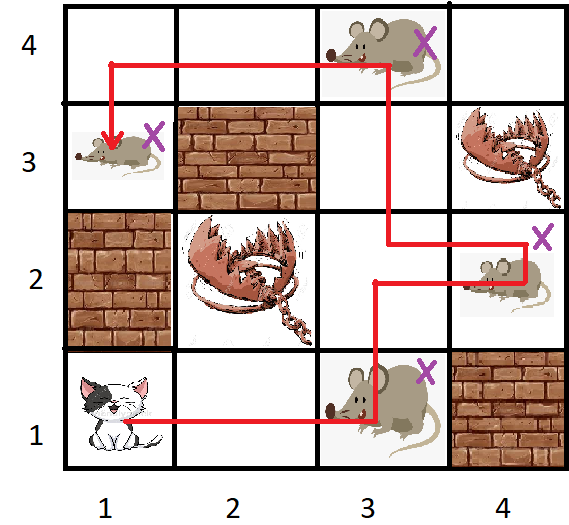
\includegraphics[width=\linewidth]{fig/A3/cat_06_sol.png}
    \caption{\textbf{Plan for problem 6}}
    \label{fig:cat_06_sol}
\end{figure}

\end{multicols}

In this problem additional were added to the world. The problem instance can be seen on figure \ref{fig:cat_06}. 

The objects that appear in the problem are: a cat, four mice, three walls, two traps and 16 squares.

\lstinputlisting[caption=Problem 6: objects, linerange=1-13, firstnumber=1]{../planning/cat-p06.pddl}

The goal, the initial state of the cat, and the adjacency relationships between the squares are unchanged. The initial positions of the mice, walls and traps are expressed in the following way:

\lstinputlisting[caption={Problem 6: initial location of the mice, walls and traps}, linerange=45-58, firstnumber=45]{../planning/cat-p06.pddl}


The goal of the problem is updated to include all four mice:

\lstinputlisting[caption=Problem 6: goal, linerange=61-61, firstnumber=61]{../planning/cat-p06.pddl}


\subsubsection{Result}

One should type the following line to run the example: 

\begin{lstlisting}[numbers=none]
fd cat-trap.pddl cat-p06.pddl --heuristic "h=ff( )" --search "astar(h)"
\end{lstlisting}

The program prints the following solution:

\lstinputlisting[caption=Output plan]{../planning/cat-p06-plan.txt}

Figure \ref{fig:cat_06_sol} visualizes the resulted plan. The cat takes a counterclockwise turn around the two walls and the neighboring trap. While taking this path, the cat eats the closest mice along the way.








\subsection{Disabling traps}

Until now the traps were equivalent to walls. Now a new ability is introduced for the cat: to disable the traps. To achieve this, the cat must grab a mouse, bring it next to the trap, then it must drop it onto the trap. This way the mouse is killed and the trap is disabled. Thus the cat can move freely to the square of the trap. While the cat is holding a mouse in its mouth, it cannot eat another mouse.


\subsubsection{Domain}

To define the new ability of the cat, additional actions are introduced: grabbing a mouse and disabling the trap with it.

A new predicate is introduced, \verb|has|, which specifies that an object has another object. A cat having a mouse means that the mouse is grabbed by the cat.

\lstinputlisting[caption=Domain: predicates, linerange=4-9, firstnumber=4]{../planning/cat-grab.pddl}

The \verb|move| and \verb|eat| actions remain unchanged.

The \verb|grab| action is introduced. Before grabbing a mouse, the cat must be alive, the cat and the mouse must be in the same square, and the cat should not hold another mouse in its mouth (because there is no place for 2 mice in his mouth). Grabbing a mouse means to remove it from the square and to attach it to the cat.

\lstinputlisting[caption=Domain: the grab action, linerange=40-52, firstnumber=40]{../planning/cat-grab.pddl}

The \verb|disable-trap | action is also introduced. Its precondition requires an alive cat which stands on a square adjacent with the square of the trap, moreover the cat must have grabbed a mouse. Disabling a trap with a mouse means to detach the mouse from the cat, to remove the trap from the square and to mark the mouse dead.

\lstinputlisting[caption=Domain: the disable-trap action, linerange=54-68, firstnumber=54]{../planning/cat-grab.pddl}


\subsubsection{Problem 7}

\begin{minipage}{\textwidth}
\begin{multicols}{2}

\begin{figure}[H]
    \centering
    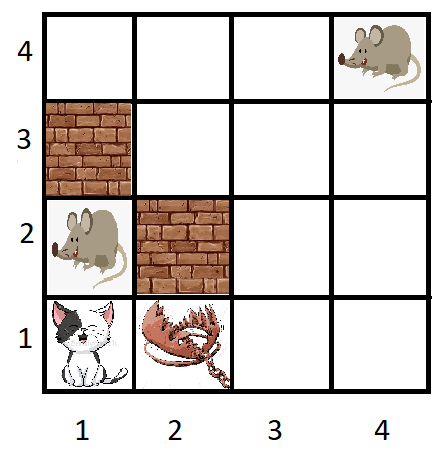
\includegraphics[width=\linewidth]{fig/A3/cat_07.png}
    \caption{\textbf{Problem 7:} Disabling a trap}
    \label{fig:cat_07}
\end{figure}

\columnbreak

\begin{figure}[H]
    \centering
    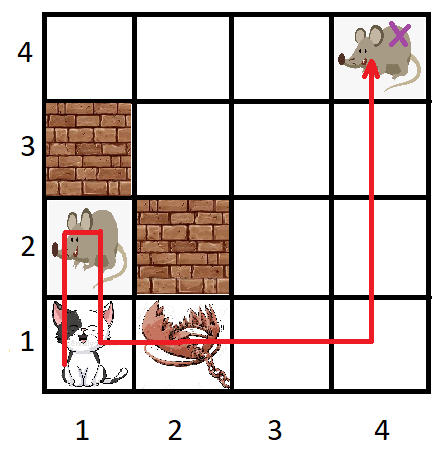
\includegraphics[width=\linewidth]{fig/A3/cat_07_sol.png}
    \caption{\textbf{Plan for problem 7:} The mouse at (2,1) does not have a purple 'x', which means that it was not eaten by the cat, instead it was grabbed by the cat and dropped at the next trap.}
    \label{fig:cat_07_sol}
\end{figure}

\end{multicols}
\medskip
\end{minipage}

In this problem the cat cannot reach the second mouse using only the \verb|move| and \verb|grab| actions because it is surrounded by a wall and a trap. Thus its only possibility is to grab the closest mouse and disable the trap with it. The problem instance can be seen on figure \ref{fig:cat_07}. 

The objects that appear in the problem are: a cat, two mice, two walls, a trap and 16 squares.

\lstinputlisting[caption=Problem 7: objects, linerange=1-13, firstnumber=1]{../planning/cat-p07.pddl}

The initial state of the cat, and the adjacency relationships between the squares are unchanged. The initial positions of the mice, walls and traps are expressed in the following way:

\lstinputlisting[caption={Problem 7: initial location of the mice, walls and traps}, linerange=45-54, firstnumber=45]{../planning/cat-p07.pddl} 


The goal of the problem is updated to include all two mice:

\lstinputlisting[caption=Problem 7: goal, linerange=58-58, firstnumber=58]{../planning/cat-p07.pddl}


\subsubsection{Result}

One should type the following line to run the example: 

\begin{lstlisting}[numbers=none]
fd cat-grab.pddl cat-p07.pddl --heuristic "h=ff( )" --search "astar(h)"
\end{lstlisting}

The program prints the following solution:

\lstinputlisting[caption=Output plan]{../planning/cat-p07-plan.txt}

Figure \ref{fig:cat_07_sol} visualizes the resulted plan. The cat grabs the closest mouse and disables the trap with it. Then it goes to the next mouse on the shortest path and eats it.







\subsection{Extending the world}

For making the problems harder, we created a bigger world, containing 36 squares. 

The adjacency relationships between the squares are defined in the following way:

\lstinputlisting[caption=Adjacency relationships for the 6x6 world, linerange=17-79, firstnumber=17]{../planning/cat-p08.pddl}

For the upcoming problems the \verb|cat-grab.pddl| domain is used.


\subsubsection{Problem 8}

\begin{minipage}{\textwidth}
\begin{multicols}{2}

\begin{figure}[H]
    \centering
    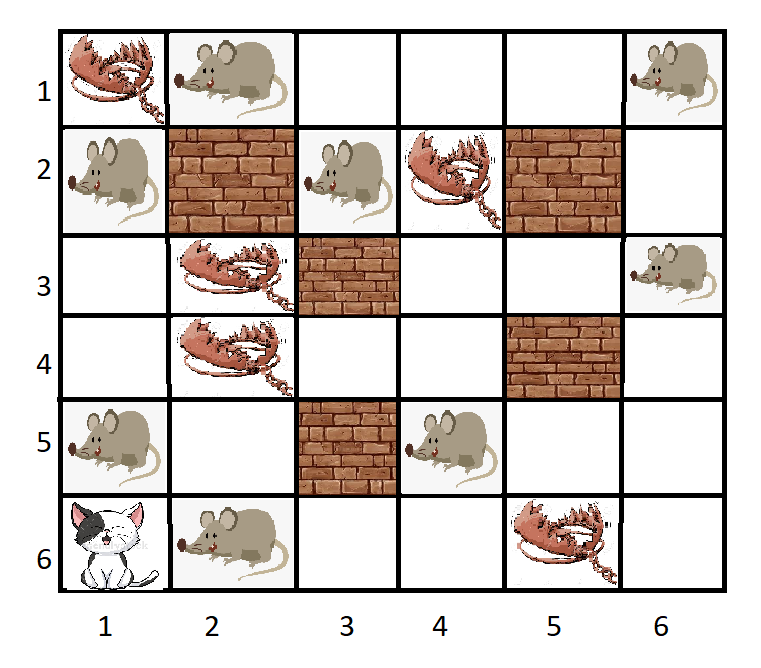
\includegraphics[width=\linewidth]{fig/A3/cat_08.png}
    \caption{\textbf{Problem 8:} Catch mice, avoid/disable traps, and avoid walls in a 6x6 world}
    \label{fig:cat_08}
\end{figure}

\columnbreak

\begin{figure}[H]
    \centering
    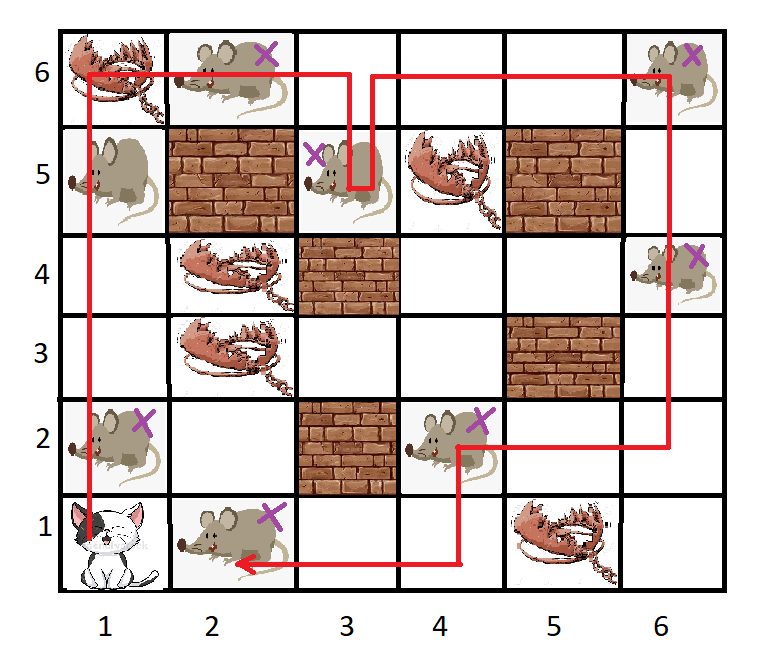
\includegraphics[width=\linewidth]{fig/A3/cat_08_sol.png}
    \caption{\textbf{Plan for problem 8}}
    \label{fig:cat_08_sol}
\end{figure}

\end{multicols}
\smallskip
\end{minipage}

This problem is an example of a 6x6 world where the agent must use all of its actions to achieve the goal efficiently. The problem instance can be seen on figure \ref{fig:cat_08}. 

The objects that appear in the problem are: a cat, eight mice, five walls, five traps and 36 squares.

\lstinputlisting[caption=Problem 8: objects, linerange=1-15, firstnumber=1]{../planning/cat-p08.pddl}

The initial state of the cat, and the adjacency relationships between the squares are unchanged. The initial positions of the mice, walls and traps are expressed in the following way:

\lstinputlisting[caption={Problem 8: initial location of the mice, walls and traps}, linerange=85-107, firstnumber=85]{../planning/cat-p08.pddl} 

 
The goal of the problem is updated to include all mice:

\lstinputlisting[caption=Problem 8: goal, linerange=111-111, firstnumber=111]{../planning/cat-p08.pddl}


\subsubsection{Result}

One should type the following line to run the example: 

\begin{lstlisting}[numbers=none]
fd cat-grab.pddl cat-p08.pddl --heuristic "h=ff( )" --search "astar(h)"
\end{lstlisting}

The program prints the following solution:

\lstinputlisting[caption=Output plan]{../planning/cat-p08-plan.txt}

Figure \ref{fig:cat_08_sol} visualizes the resulted plan. The cat does a big clockwise turn. It eats the first mouse. When it reaches the second, instead of eating it and turning around, the cat grabs the mouse and disables the trap. Then by passing through the trap, the cat can move forward to eat all the other mice, by moving each time on the shortest path towards the closest mouse. 



\subsubsection{Problem 9}

\begin{multicols}{2}

\begin{figure}[H]
    \centering
    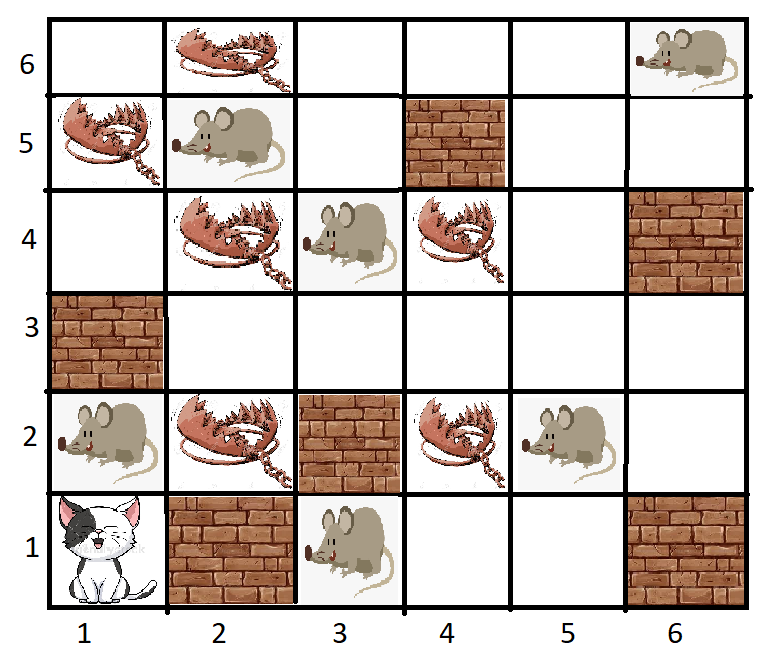
\includegraphics[width=\linewidth]{fig/A3/cat_09.png}
    \caption{\textbf{Problem 9:} Catch mice, avoid/disable traps, and avoid walls in a 6x6 world}
    \label{fig:cat_09}
\end{figure}

\columnbreak

\begin{figure}[H]
    \centering
    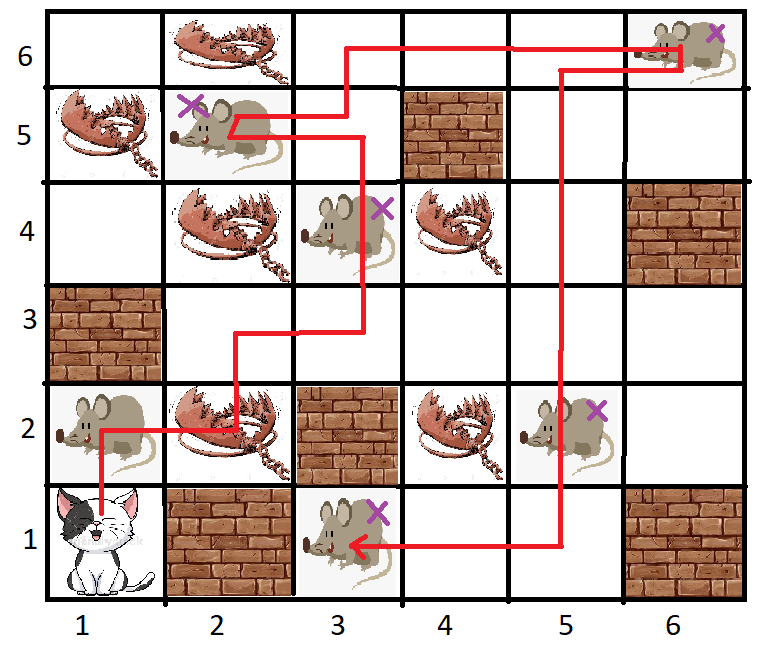
\includegraphics[width=\linewidth]{fig/A3/cat_09_sol.png}
    \caption{\textbf{Plan for problem 9}}
    \label{fig:cat_09_sol}
\end{figure}

\end{multicols}

The scenario described by the problem instance is another example for the case when the cat is obliged to disable a trap using a mouse. The problem instance can be seen on figure \ref{fig:cat_09}. 

The objects that appear in the problem are: a cat, six mice, six walls, six traps and 36 squares.

\lstinputlisting[caption=Problem 9: objects, linerange=1-15, firstnumber=1]{../planning/cat-p09.pddl}

The initial state of the cat, and the adjacency relationships between the squares are unchanged. The initial positions of the mice, walls and traps are expressed in the following way:

\lstinputlisting[caption={Problem 9: initial location of the mice, walls and traps}, linerange=85-107, firstnumber=85]{../planning/cat-p09.pddl} 

 
The goal of the problem is updated to include all mice:

\lstinputlisting[caption=Problem 9: goal, linerange=110-110, firstnumber=110]{../planning/cat-p09.pddl} 


\subsubsection{Result}

One should type the following line to run the example: 

\begin{lstlisting}[numbers=none]
fd cat-grab.pddl cat-p09.pddl --heuristic "h=ff( )" --search "astar(h)"
\end{lstlisting}

The program prints the following solution:

\lstinputlisting[caption=Output plan]{../planning/cat-p09-plan.txt}

Figure \ref{fig:cat_09_sol} visualizes the resulted plan. 

The mice marked with a purple X were eaten by the cat, the other one was 'thrown' into the trap, so the cat could pass through it.

As we can see, in the first step, the cat having no other option, it had to grab the mouse at (2,1) and throw it into the trap at (2,2) so that it could go forward to eat the other mice.



\subsubsection{Problem 10}
\label{sec:prob_10}

\begin{multicols}{2}

\begin{figure}[H]
    \centering
    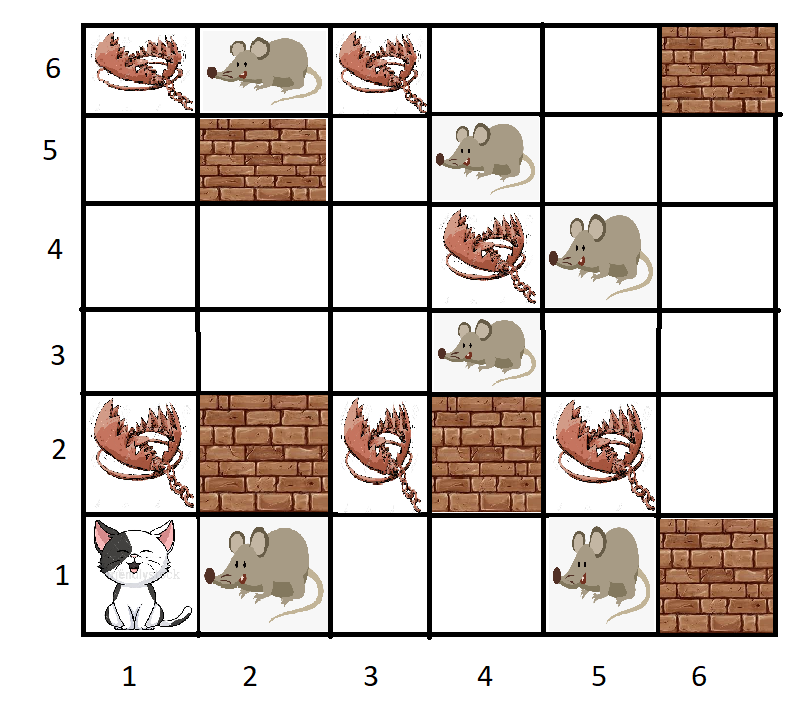
\includegraphics[width=\linewidth]{fig/A3/cat_10.png}
    \caption{\textbf{Problem 10:} Catch mice, avoid/disable traps, and avoid walls in a 6x6 world}
    \label{fig:cat_10}
\end{figure}

\columnbreak

\begin{figure}[H]
    \centering
    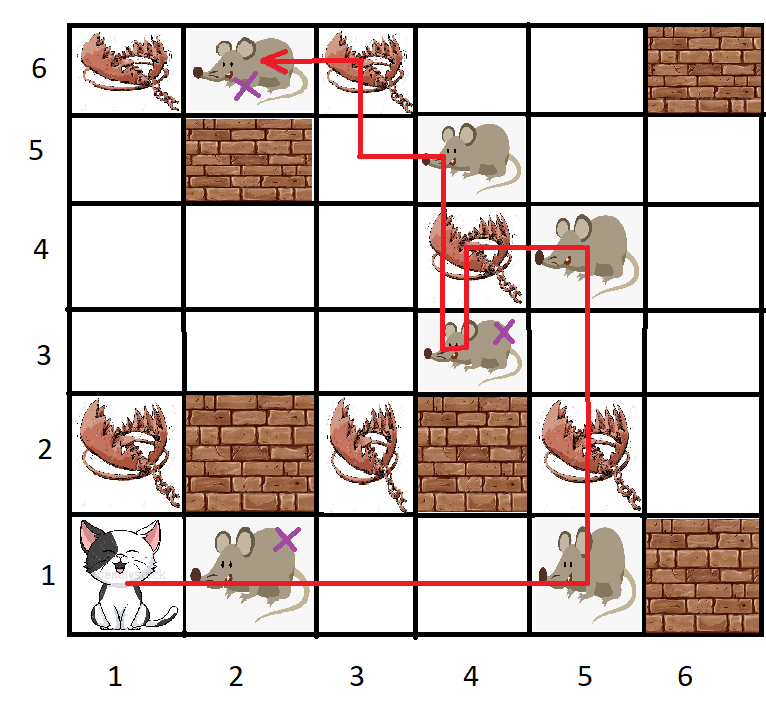
\includegraphics[width=\linewidth]{fig/A3/cat_10_sol.png}
    \caption{\textbf{Plan for problem 10}}
    \label{fig:cat_10_sol}
\end{figure}

\end{multicols}

This problem is an example for the case when the cat is obliged to disable a trap using a mouse. However now the cat must choose between multiple traps, to disable one or more of them. The problem instance can be seen on figure \ref{fig:cat_10}. 

The objects that appear in the problem are: a cat, six mice, five walls, six traps and 36 squares.

\lstinputlisting[caption=Problem 10: objects, linerange=1-15, firstnumber=1]{../planning/cat-p10.pddl}

The initial state of the cat, and the adjacency relationships between the squares are unchanged. The initial positions of the mice, walls and traps are expressed in the following way:

\lstinputlisting[caption={Problem 10: initial location of the mice, walls and traps}, linerange=85-106, firstnumber=85]{../planning/cat-p10.pddl} 

 
The goal of the problem is updated to include all mice:

\lstinputlisting[caption=Problem 10: goal, linerange=110-110, firstnumber=110]{../planning/cat-p10.pddl} 


\subsubsection{Result} 
\label{sec:prob_10_res}

One should type the following line to run the example: 

\begin{lstlisting}[numbers=none]
fd cat-grab.pddl cat-p10.pddl --heuristic "h=ff( )" --search "astar(h)"
\end{lstlisting}

The program prints the following solution:

\lstinputlisting[caption=Output plan]{../planning/cat-p10-plan.txt}

Figure \ref{fig:cat_10_sol} visualizes the resulted plan. The cat is trapped in the first row, so it is forced to throw a mouse in one of the traps from the second row. It chooses the last one, and it eats the closest mouse. Similarly in the sixth row, the mouse is place between two traps and a wall, so the cat is forced to disable one of the traps, using a mouse.










\subsection{Adding costs to actions}

To influence the behavior of the agent one should assign priorities to actions. The agent would choose from two potential actions the one which has a higher priority i.e. has a lower cost.

We will use the world described in problem 10 and modify the action costs in the domain.

\subsubsection{Problem 11}

This problem is the copy of problem 10. The instance can be seen on figure \ref{fig:cat_10}. The only difference is that we introduce the \verb|total-cost| function.

Initializing the total cost to 0:

\lstinputlisting[caption=Problem 11: total cost, linerange=108-108, firstnumber=108]{../planning/cat-p11.pddl} 

Specifying to minimize the total cost:

\lstinputlisting[caption=Problem 11: metric, linerange=114-114, firstnumber=114]{../planning/cat-p11.pddl} 


\subsubsection{Domain - Uniform}

The \verb|cat-weight-uniform.pddl| file defines a domain which works the same as \verb|cat-grab.pddl| because the weight of each action is equal to 1, i.e. each action has uniform cost. Therefore the priority is tho eat all the mice with the least number of actions.

The requirements are updated to enable costs to actions:

\lstinputlisting[caption=Domain - Uniform: requirements, linerange=2-2, firstnumber=2]{../planning/cat-weight-uniform.pddl} 

The \verb|total-cost| function is added:

\lstinputlisting[caption=Domain - Uniform: functions, linerange=11-13, firstnumber=11]{../planning/cat-weight-uniform.pddl} 

In the \verb|:effect| part of each action a uniform cost is added. An example is:

\lstinputlisting[caption=Domain - Uniform: adding uniform cost, linerange=54-58, firstnumber=54]{../planning/cat-weight-uniform.pddl} 


\subsubsection{Result}

One should type the following line to run the example: 

\begin{lstlisting}[numbers=none]
fd cat-weight-uniform.pddl cat-p11.pddl --heuristic "h=ff( )" --search "astar(h)"
\end{lstlisting}

The program prints the exact same output as for problem 10 described in section \ref{sec:prob_10_res}. The cat chose to eat some mice, and chose to throw some mice into the traps even if it wasn't forced to do it (e.g at (4,4)). 




\subsubsection{Domain - Eat Priority}

In this domain the cost of eating a mouse is 1, the cost of disabling a trap is 10000 and the cost of all other actions is 1000. This way we tell the planner that it should eat mice and it should disable traps only if it is forced to do it.

\subsubsection{Result}

One should type the following line to run the example: 

\begin{lstlisting}[numbers=none]
fd cat-weight-eat.pddl cat-p11.pddl --heuristic "h=ff( )" --search "astar(h)"
\end{lstlisting}

The program prints the following solution:

\lstinputlisting[caption=Output plan]{../planning/cat-p11-plan-eat.txt}

One can observe that the agent prioritized the eating of mice over the disabling of the traps. The number of actions does not matter in this case. The cat disabled only those two traps which blocks it from reaching the next mouse. When using the uniform domain, an additional third trap (at (4,4)) was also disabled to reduce the number of actions. Now this trap is remained enable because the low priority of the corresponding action.  




\subsubsection{Domain - Trap Priority}

In this domain the cost for disabling a trap is 1, the cost of eating a mouse is 10000 and the cost of all other actions is 1000. This way we tell the planner that it should disable traps and it should not eat mice, unless there are no more traps.


\subsubsection{Result}

One should type the following line to run the example: 

\begin{lstlisting}[numbers=none]
fd cat-weight-trap.pddl cat-p11.pddl --heuristic "h=ff( )" --search "astar(h)"
\end{lstlisting}

The program prints the following solution:

\lstinputlisting[caption=Output plan]{../planning/cat-p11-plan-trap.txt}

One can observe that the agent prioritized the disabling of the traps instead of eating all the mice as fast as possible. It disabled all the traps and did not eat any mice.
